\chapter{Fundamentação Teórica}
\label{cap:fundamentacao}

% -----------------------------------------------------------------
% Fio argumentativo do capítulo (funil até a lacuna):
%
%   2.1  Apresenta o contexto industrial: processo produtivo do
%        fio esmaltado, das etapas de fundição/laminação do
%        vergalhão até o esmaltamento final.
%   2.2  Estabelece que o problema é real e multifatorial,
%        ancorado em Karabay (2018) e Demiri (2014). Cobre os
%        modos de falha do fio nu e do esmaltado. RQ5.
%   2.3  Inventaria os dados produzidos pela operação que
%        sustentam a análise da dissertação e destaca a
%        ausência de rótulo de causa.
%   2.4  Mostra a tradição de apoio à decisão técnica e suas
%        limitações diante de dados sensoriais modernos.
%   2.5  Apresenta a primeira família de técnicas (anomalias
%        em séries operacionais) que sustenta o Pilar EQ. RQ1.
%   2.6  Apresenta a segunda família (estatística histórica por
%        lote, fornecedor, máquina) que sustenta o Pilar MP. RQ3.
%   2.7  Discute a integração das duas famílias e a
%        explicabilidade, apontando a lacuna que o WireSense
%        ocupa. RQ2 e RQ4.
%
% Protocolo da revisão sistemática:
%   docs/dissertacao/protocolo_revisao.md
% Sementes para bootstrap:
%   Chandola et al. (2009), Pang et al. (2021), Liu et al. (2008).
% -----------------------------------------------------------------

Este capítulo apresenta o referencial teórico que sustenta a dissertação. A construção do referencial começa pela caracterização do domínio em que o problema se manifesta: o processo produtivo de fios esmaltados de cobre e alumínio, com suas etapas sucessivas de fundição, trefilação e esmaltamento. Nesse contexto, descrevem-se os mecanismos pelos quais um rompimento pode ser produzido, tanto os de origem metalúrgica, ligados à matéria-prima, quanto os de origem operacional, ligados à interação do fio com o equipamento, e inventariam-se os dados que a operação registra ao longo das linhas, incluindo a ausência de rótulo padronizado de causa.

Estabelecido o domínio, o capítulo avança para a revisão das técnicas que apoiam a decisão técnica em manufatura. A discussão começa pela tradição de diagnóstico de falhas, que reúne instrumentos como FMEA, análise de causa raiz e controle estatístico de processo. Esses instrumentos são amplamente utilizados na indústria, mas apresentam limites diante de dados sensoriais em alta frequência. Em seguida, examinam-se duas famílias de técnicas orientadas a dados: a detecção de anomalias em séries operacionais multivariadas e a análise estatística histórica de falhas segmentada por lote, material, fornecedor e máquina. O capítulo encerra discutindo estratégias de integração entre essas famílias e o papel da explicabilidade em ambiente produtivo, apontando a lacuna que este trabalho busca abordar.


\section{Contexto Industrial}
\label{sec:contexto_industrial}

Esta seção apresenta o contexto industrial em que o problema desta pesquisa se manifesta. A fabricação de fios esmaltados de cobre e alumínio é um processo contínuo que parte do vergalhão recebido como matéria-prima e o transforma, ao longo de etapas sucessivas, em fio pronto para aplicações de enrolamento elétrico em motores, transformadores e demais componentes magnéticos \cite{demiri2014enamel,niu2024superior,caruso2022novel}. As subseções seguintes descrevem as três etapas principais da cadeia produtiva. A primeira aborda a produção do vergalhão pelo fornecedor, origem da matéria-prima utilizada pela fábrica. A segunda trata da trefilação primária, responsável pela transformação do vergalhão em fio nu na linha da fábrica. A terceira apresenta o esmaltamento, etapa que aplica as camadas de isolamento elétrico necessárias para o uso final do produto.


\subsection{Fundição para criação da matéria-prima}
\label{subsec:fundicao}

A Figura~\ref{fig:fluxo_vergalhao} apresenta o fluxo simplificado da produção do vergalhão de cobre por lingotamento contínuo e laminação. O processo inicia com cátodos de cobre eletro-refinado, que são carregados no forno de fusão. Após a fusão, o cobre líquido é transferido por canal para o forno de retenção e, em seguida, conduzido à máquina de lingotamento contínuo. Na rota Southwire, a máquina de lingotamento utiliza uma roda de aço com canal periférico, fechado por uma cinta metálica, formando a cavidade de solidificação. Durante a rotação, o cobre é resfriado com água e forma uma barra contínua \cite{cuypers1987continuous}.

\begin{figure}[htbp]
    \centering
    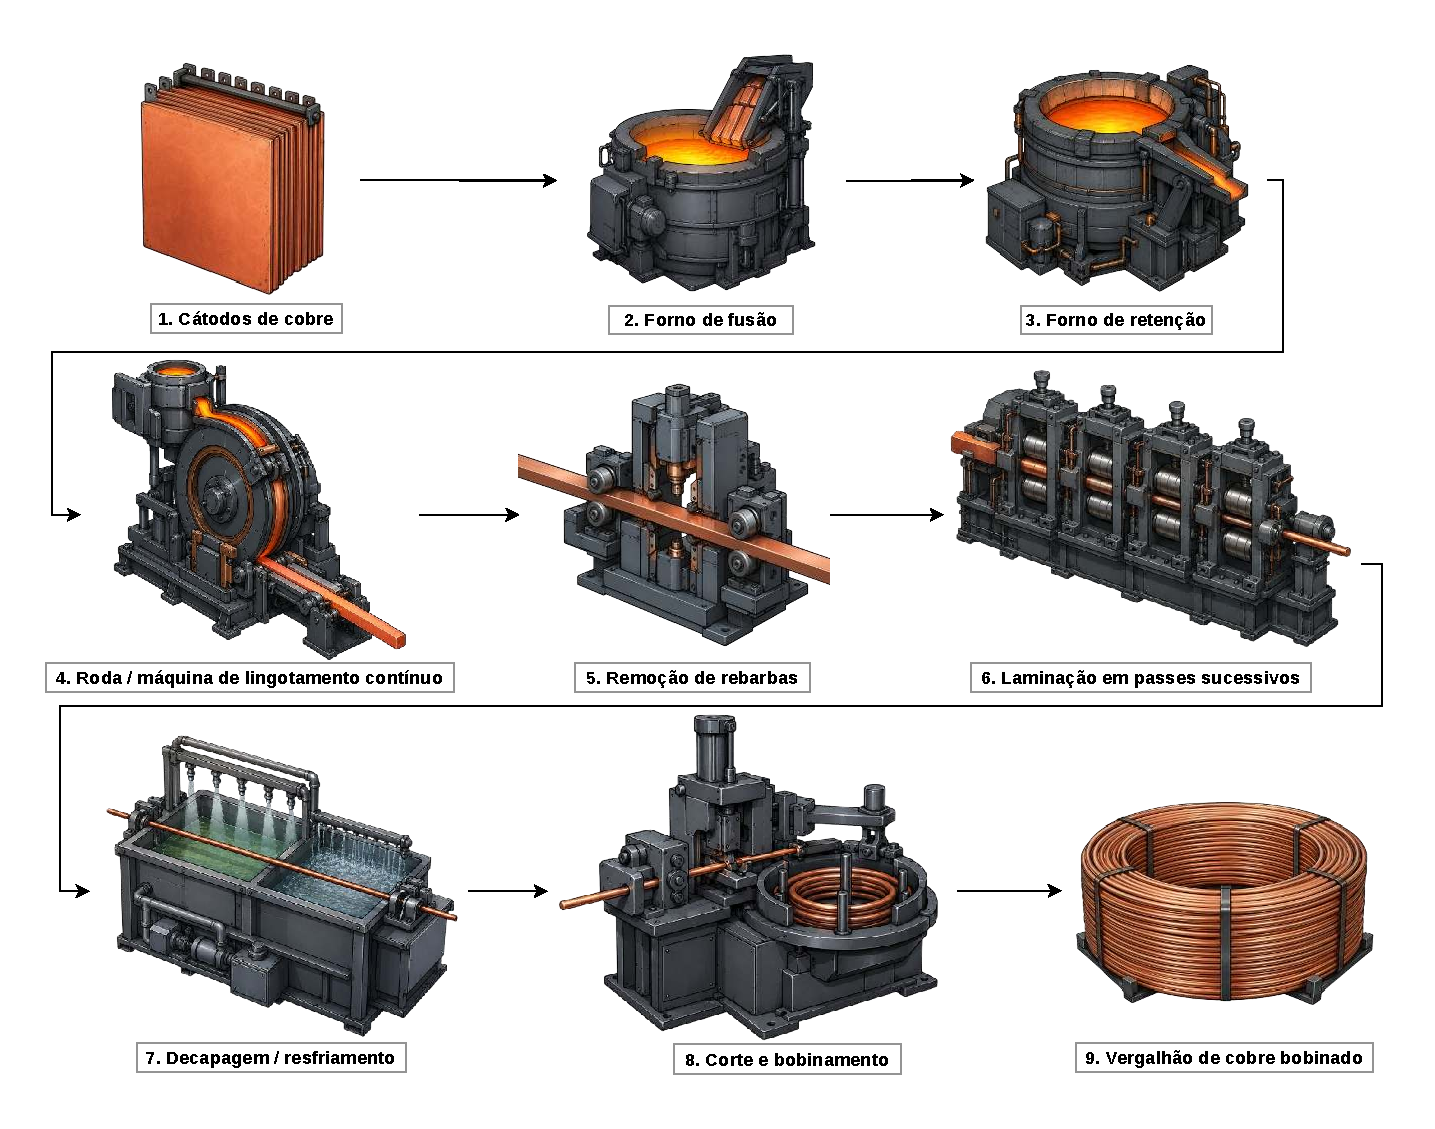
\includegraphics[width=\textwidth]{Figuras/fundicao.pdf}
    \caption{Fluxo simplificado da produção do vergalhão de cobre por lingotamento contínuo e laminação.}
    \label{fig:fluxo_vergalhao}
    \fonte{Adaptado de \citeonline{cuypers1987continuous}.}
\end{figure}

Após o lingotamento, a barra contínua passa por uma etapa de remoção de rebarbas antes de seguir para a laminação. Em seguida, a barra é processada em um trem de laminação com múltiplos passes, responsável pela redução progressiva da seção até a obtenção do diâmetro especificado para o vergalhão. As linhas de \emph{Continuous Casting and Rolling} (CCR) são compostas por forno de fusão, forno de retenção, unidade de lingotamento, trem de laminação, sistema de decapagem e bobinador \cite{cuypers1987continuous}.

Na sequência final, o vergalhão passa por decapagem e resfriamento para remoção da camada superficial de óxidos e preparação do produto. Por fim, o material é cortado e bobinado, originando o vergalhão de cobre. Essa sequência corresponde à rota \sigla{CCR}, na qual o cobre é continuamente fundido, solidificado, laminado, decapado e bobinado. O vergalhão assim produzido constitui a matéria-prima de entrada da fábrica de fios, onde será transformado em fio nu pela trefilação primária.


\subsection{Trefilação primária}
\label{subsec:trefilacao}

A trefilação primária recebe o vergalhão fornecido por terceiros e o transforma em fio de cobre ou alumínio nu próprio para alimentar a linha de esmaltação. O processo se dá em uma máquina de trefilação que executa uma sequência de passes em fieiras, reduzindo o diâmetro a cada estágio até o calibre intermediário desejado \cite{wright2011wire}. Na fábrica de fios analisada, o vergalhão é adquirido de múltiplos fornecedores. Para cobre, a linha produz três bitolas iniciais distintas, cada uma destinada a famílias específicas de produtos. Para alumínio, há uma única bitola intermediária. A Figura~\ref{fig:pretrefilacao} ilustra a etapa na fábrica analisada.

\begin{figure}[htbp]
    \centering
    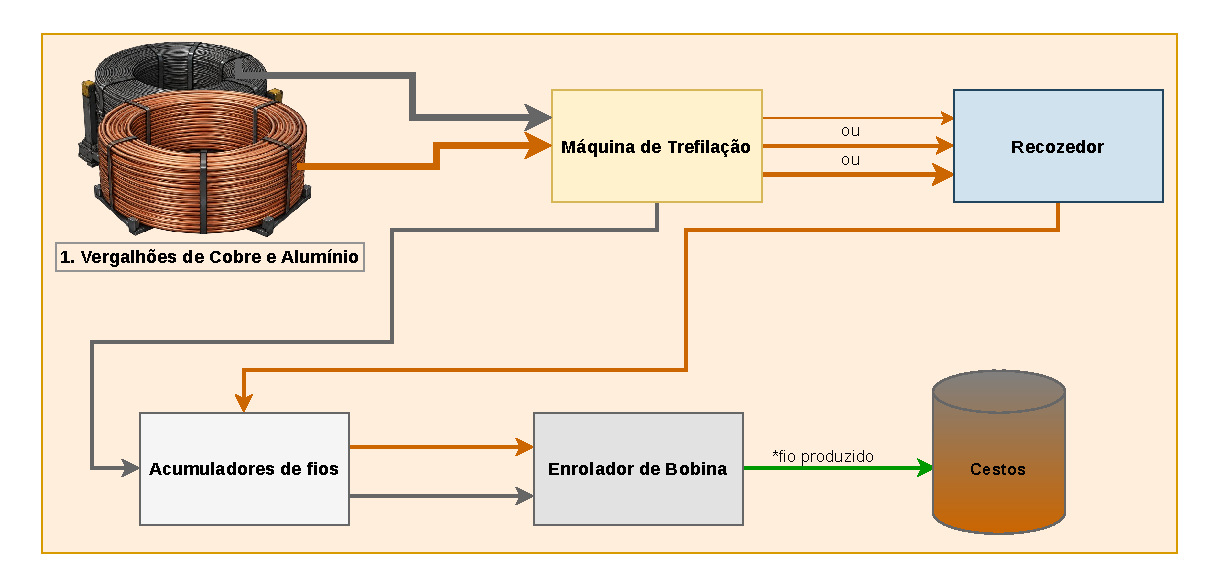
\includegraphics[width=\textwidth]{Figuras/pretrefilacao.pdf}
    \caption{Etapa de trefilação primária na fábrica analisada.}
    \label{fig:pretrefilacao}
    \fonte{Elaborado pelo autor (\the\year).}
\end{figure}

O cobre passa, ainda nesta linha, por uma etapa de recozimento posterior à trefilação. Essa etapa restaura a ductilidade reduzida pelo trabalho a frio dos múltiplos passes e recupera a condutividade elétrica degradada durante a deformação \cite{wright2011wire}. Defeitos internos como \emph{central bursts} e fissuras em \emph{chevron}\footnote{Termos técnicos para a mesma família de descontinuidades internas que se formam no eixo do fio durante a trefilação, resultantes de tensões hidrostáticas trativas no núcleo da seção. \emph{Central burst} enfatiza a localização do defeito no centro do fio, enquanto \emph{chevron} alude ao formato de v que essas fissuras apresentam em corte longitudinal.} formados nos primeiros passes podem permanecer ocultos e só se manifestar em estágios posteriores, reforçando a necessidade de recozimentos inter-operacionais, com tempo e temperatura adequados para restaurar a deformabilidade total do material \cite{zasadzinska2022defects}. O alumínio pode dispensar recozimentos intermediários em certas rotas de trefilação, desde que a sequência de reduções por passe e os parâmetros de processo sejam adequadamente definidos. Estudos com alumínio EN AW-1370 mostram a viabilidade de trefilação multiestágio com redução acumulada superior a 90\% sem tratamento de recozimento, embora o material ainda apresente encruamento progressivo ao longo dos passes \cite{rodriguez2019wiredrawing}.

O fio nu resultante da trefilação primária, seja em cobre ou em alumínio, é acondicionado em cestos identificados por lote. Essa prática preserva a rastreabilidade entre o vergalhão original e o produto trefilado e permite isolar lotes específicos quando defeitos são observados durante o esmaltamento.


\subsection{Esmaltamento}
\label{subsec:esmaltamento}

Após a trefilação primária, o fio de cobre ou alumínio nu segue para a linha de esmaltamento, etapa que aplica camadas de verniz isolante sobre a superfície do fio. O esmalte cumpre principalmente a função de insulação elétrica, condição necessária para que o fio possa ser enrolado em bobinas próximas umas das outras sem provocar curto-circuito entre espiras vizinhas. Esmaltes finos minimizam ainda o espaço ocupado pelo isolamento nas bobinas, mantêm alta rigidez dielétrica e oferecem resistência a umidade e a solventes do ambiente de operação \cite{demiri2014enamel}. A Figura~\ref{fig:esmaltamento} apresenta o fluxo da etapa na fábrica analisada.

\begin{figure}[htbp]
    \centering
    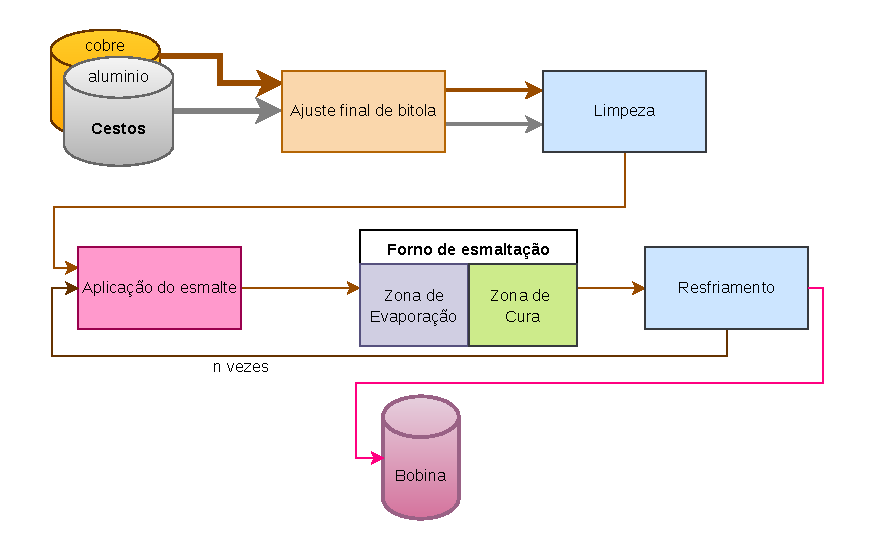
\includegraphics[width=\textwidth]{Figuras/esmaltacao.pdf}
    \caption{Fluxo da etapa de esmaltamento na fábrica analisada. \textcolor{red}{Falta melhorar cores e nomenclaturas.}}
    \label{fig:esmaltamento}
    \fonte{Elaborado pelo autor (\the\year).}
\end{figure}

Antes do início do ciclo de esmaltamento, o fio nu retirado dos cestos passa por uma etapa de ajuste final de bitola, equivalente a uma trefilação fina, seguida de uma etapa de limpeza superficial. O ciclo de esmaltamento propriamente dito combina aplicação, cura e resfriamento em sequência, repetidos até seis vezes \cite{wright2011wire}. O fio passa por um aplicador que deposita uma camada de esmalte em solução resinosa e em seguida entra no forno de esmaltação, no qual uma zona de evaporação remove o solvente e uma zona de cura completa a polimerização do filme. Após o resfriamento, o fio retorna ao aplicador para receber a próxima camada.

O aumento total de diâmetro do fio decorrente das camadas é denominado \emph{build}. A montagem física da linha é vertical, motivo pelo qual o equipamento é chamado \emph{enameling tower} \cite{wright2011wire}. Concluído o \emph{build} especificado, o fio esmaltado é bobinado em sua apresentação final. Cada uma das etapas apresentadas, no entanto, pode ser interrompida por rompimentos do fio, evento operacional cujas causas e mecanismos são examinados na Seção~\ref{sec:problema_rompimentos}.


\section{Problema de rompimentos de fios de cobre e alumínio}
\label{sec:problema_rompimentos}

% Função retórica (do esboço original): estabelecer que o problema é real e multifatorial.
% RQ5. Cobre os modos de falha do fio nu e do esmaltado, com Karabay (2018) e Demiri (2014) como ancoragem.

Um rompimento corresponde à interrupção da continuidade do fio durante a passagem pela linha de produção. Quando ocorre, a máquina para de operar, o material em curso precisa ser religado ou descartado e o ciclo produtivo é retomado após intervenção do operador. Em uma fábrica de fios esmaltados, esses eventos concentram a maior parte das paradas não programadas e impactam tanto a produtividade da linha quanto o retrabalho associado ao produto interrompido \cite{zasadzinska2022defects}. Na fábrica analisada, dados operacionais indicam projeção de perdas para 2025 da ordem de \textcolor{red}{R\$~4,2 milhões} associados a rompimentos e \textcolor{red}{R\$~2,8 milhões} a defeitos do tipo bolha. Por essa razão, o rompimento é tratado nesta dissertação como o sintoma operacional central a ser analisado.

Os rompimentos podem ocorrer em diferentes pontos da cadeia produtiva descrita na Seção~\ref{sec:contexto_industrial}. Na trefilação primária, o fio nu é submetido a múltiplos passes de redução de seção, e qualquer descontinuidade interna ou superficial pode atuar como concentrador de tensão e dar origem ao rompimento. No esmaltamento, o fio passa por aplicações sucessivas de verniz, evaporação de solvente e cura em forno, etapas em que defeitos térmicos, de aplicação ou de contaminação do filme isolante também levam à interrupção do fio. Apesar da diferença de etapa, o evento observado pelo operador é semelhante em ambos os casos: um fio rompido na linha. A inspeção direta após o evento raramente é suficiente para determinar a causa, porque mecanismos distintos produzem fenótipos semelhantes na superfície de fratura \cite{karabay2018failure}.

A literatura agrupa esses mecanismos em duas categorias principais de causa raiz: defeitos originados na matéria-prima e defeitos originados na interação do material com o equipamento \cite{karabay2018failure}. A primeira categoria inclui descontinuidades formadas nas etapas de fundição e laminação do vergalhão, e a segunda inclui danos introduzidos durante a trefilação, o transporte entre estações e a passagem pela linha de esmaltamento. Os defeitos da primeira categoria viajam embutidos no fio até serem expostos por solicitação mecânica posterior, o que torna o ponto de ruptura espacialmente desacoplado da causa de origem.

No fio nu, sete modos de falha foram identificados em análise por microscopia eletrônica de varredura e espectroscopia por energia dispersiva \cite{karabay2018failure}. O defeito de \emph{hole} resulta de extrusão excessiva do vergalhão. Cavidades de solidificação no núcleo do fio decorrem de resfriamento inadequado na roda de cristalização. Inclusões de óxido embutidas na superfície originam-se de fluxagem insuficiente ou turbulência no vazamento. O defeito conhecido como \emph{check} é causado pelo rasgamento da camada oxidada do vergalhão. O \emph{splinter} corresponde a uma lasca destacada a partir de partículas oxidadas duras em contato com o cone da fieira. O \emph{overfill} forma-se por folgas inadequadas entre os rolos da laminação do vergalhão trapezoidal. Por fim, zonas de acumulação de óxido metálico aparecem nas guias das máquinas de encordoamento. A Figura~\ref{fig:karabay_fig04} ilustra dois desses modos no fio nu de alumínio: o defeito de \emph{hole} e as cavidades de solidificação no núcleo do fio.

\begin{figure}[htbp]
    \centering
    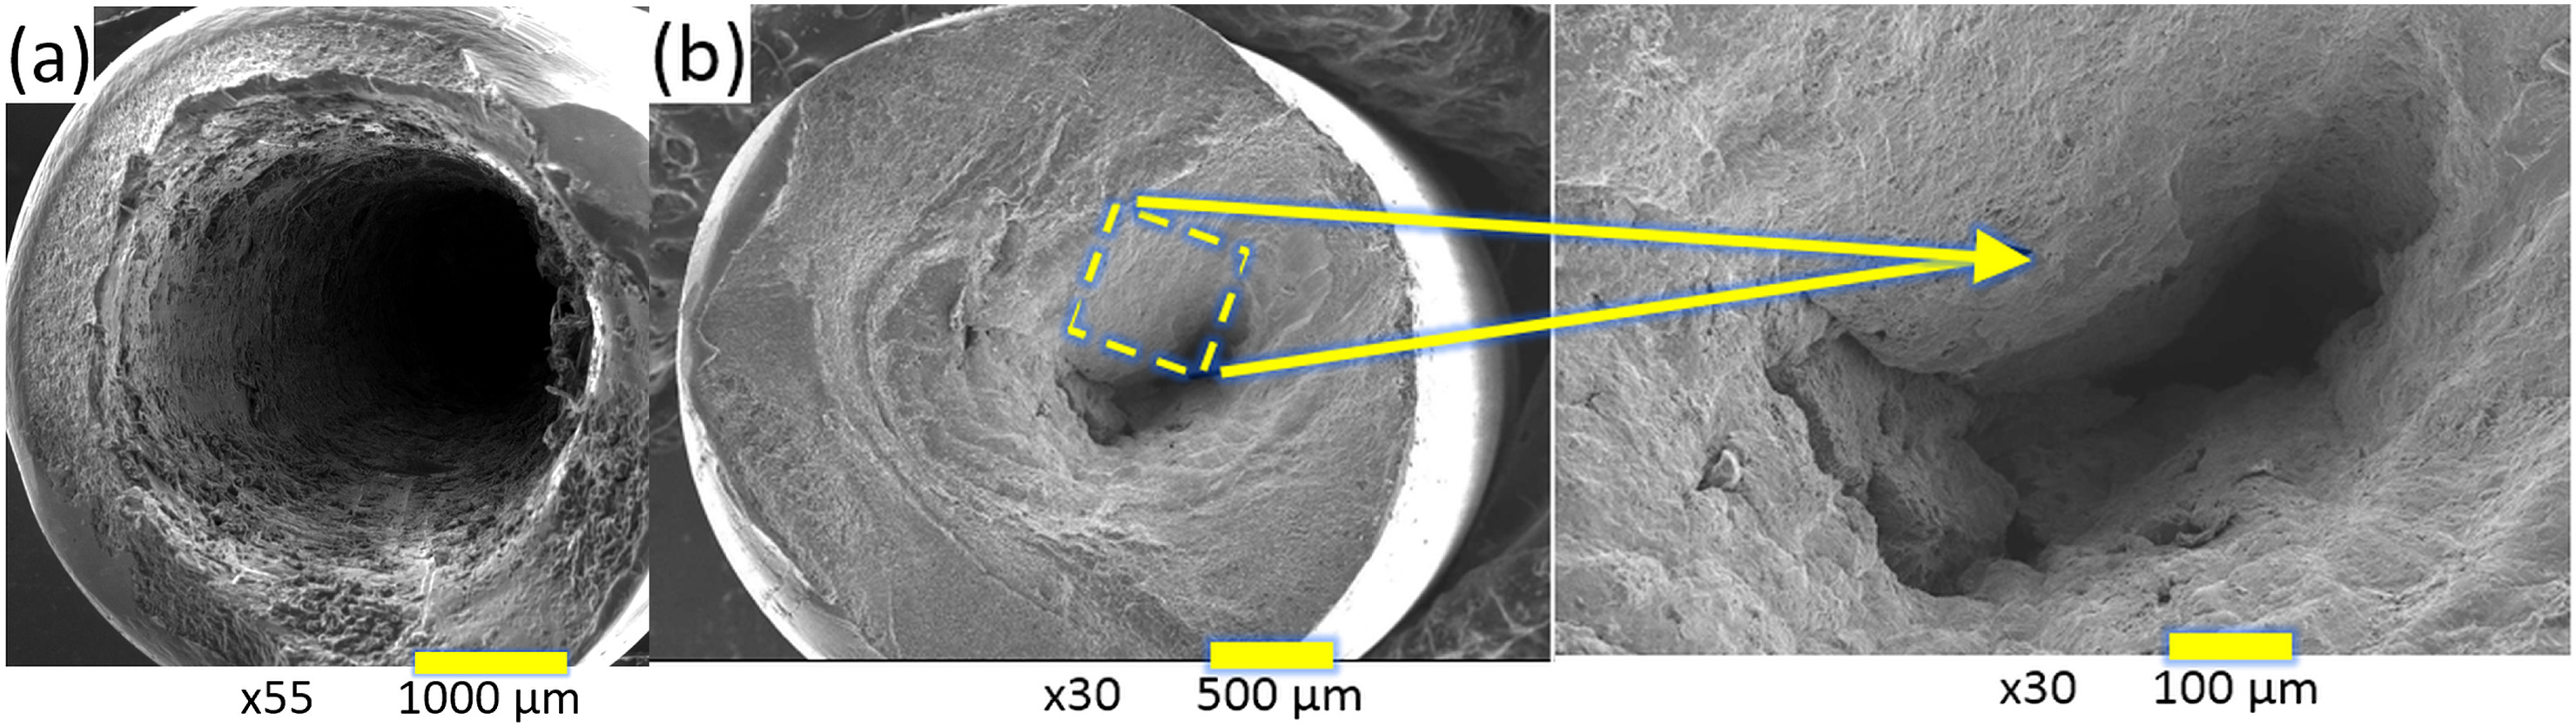
\includegraphics[width=\textwidth]{Figuras/Karabay_2018_fig04_hole_solidification.jpg}
    \caption{Defeitos metalúrgicos típicos em fio nu de alumínio. (a) Defeito de \emph{hole} no fio trefilado a partir do vergalhão AA6101. (b) Cavidades de solidificação no núcleo do fio.}
    \label{fig:karabay_fig04}
    \fonte{\citeonline{karabay2018failure}.}
\end{figure}

A esses mecanismos de origem metalúrgica somam-se ainda danos superficiais introduzidos pela trefilação propriamente dita, como riscos longitudinais associados a desgaste das fieiras, ruptura do filme lubrificante e deformação plástica de superfície por impacto de carretel \cite{wright2011wire}. A Figura~\ref{fig:karabay_fig07} ilustra um exemplo característico desse segundo grupo: uma zona de acumulação de óxido metálico formada nas guias da linha, em que tensões repetidas de flexão e torção concentram-se em região fragilizada e levam à fratura.

\begin{figure}[htbp]
    \centering
    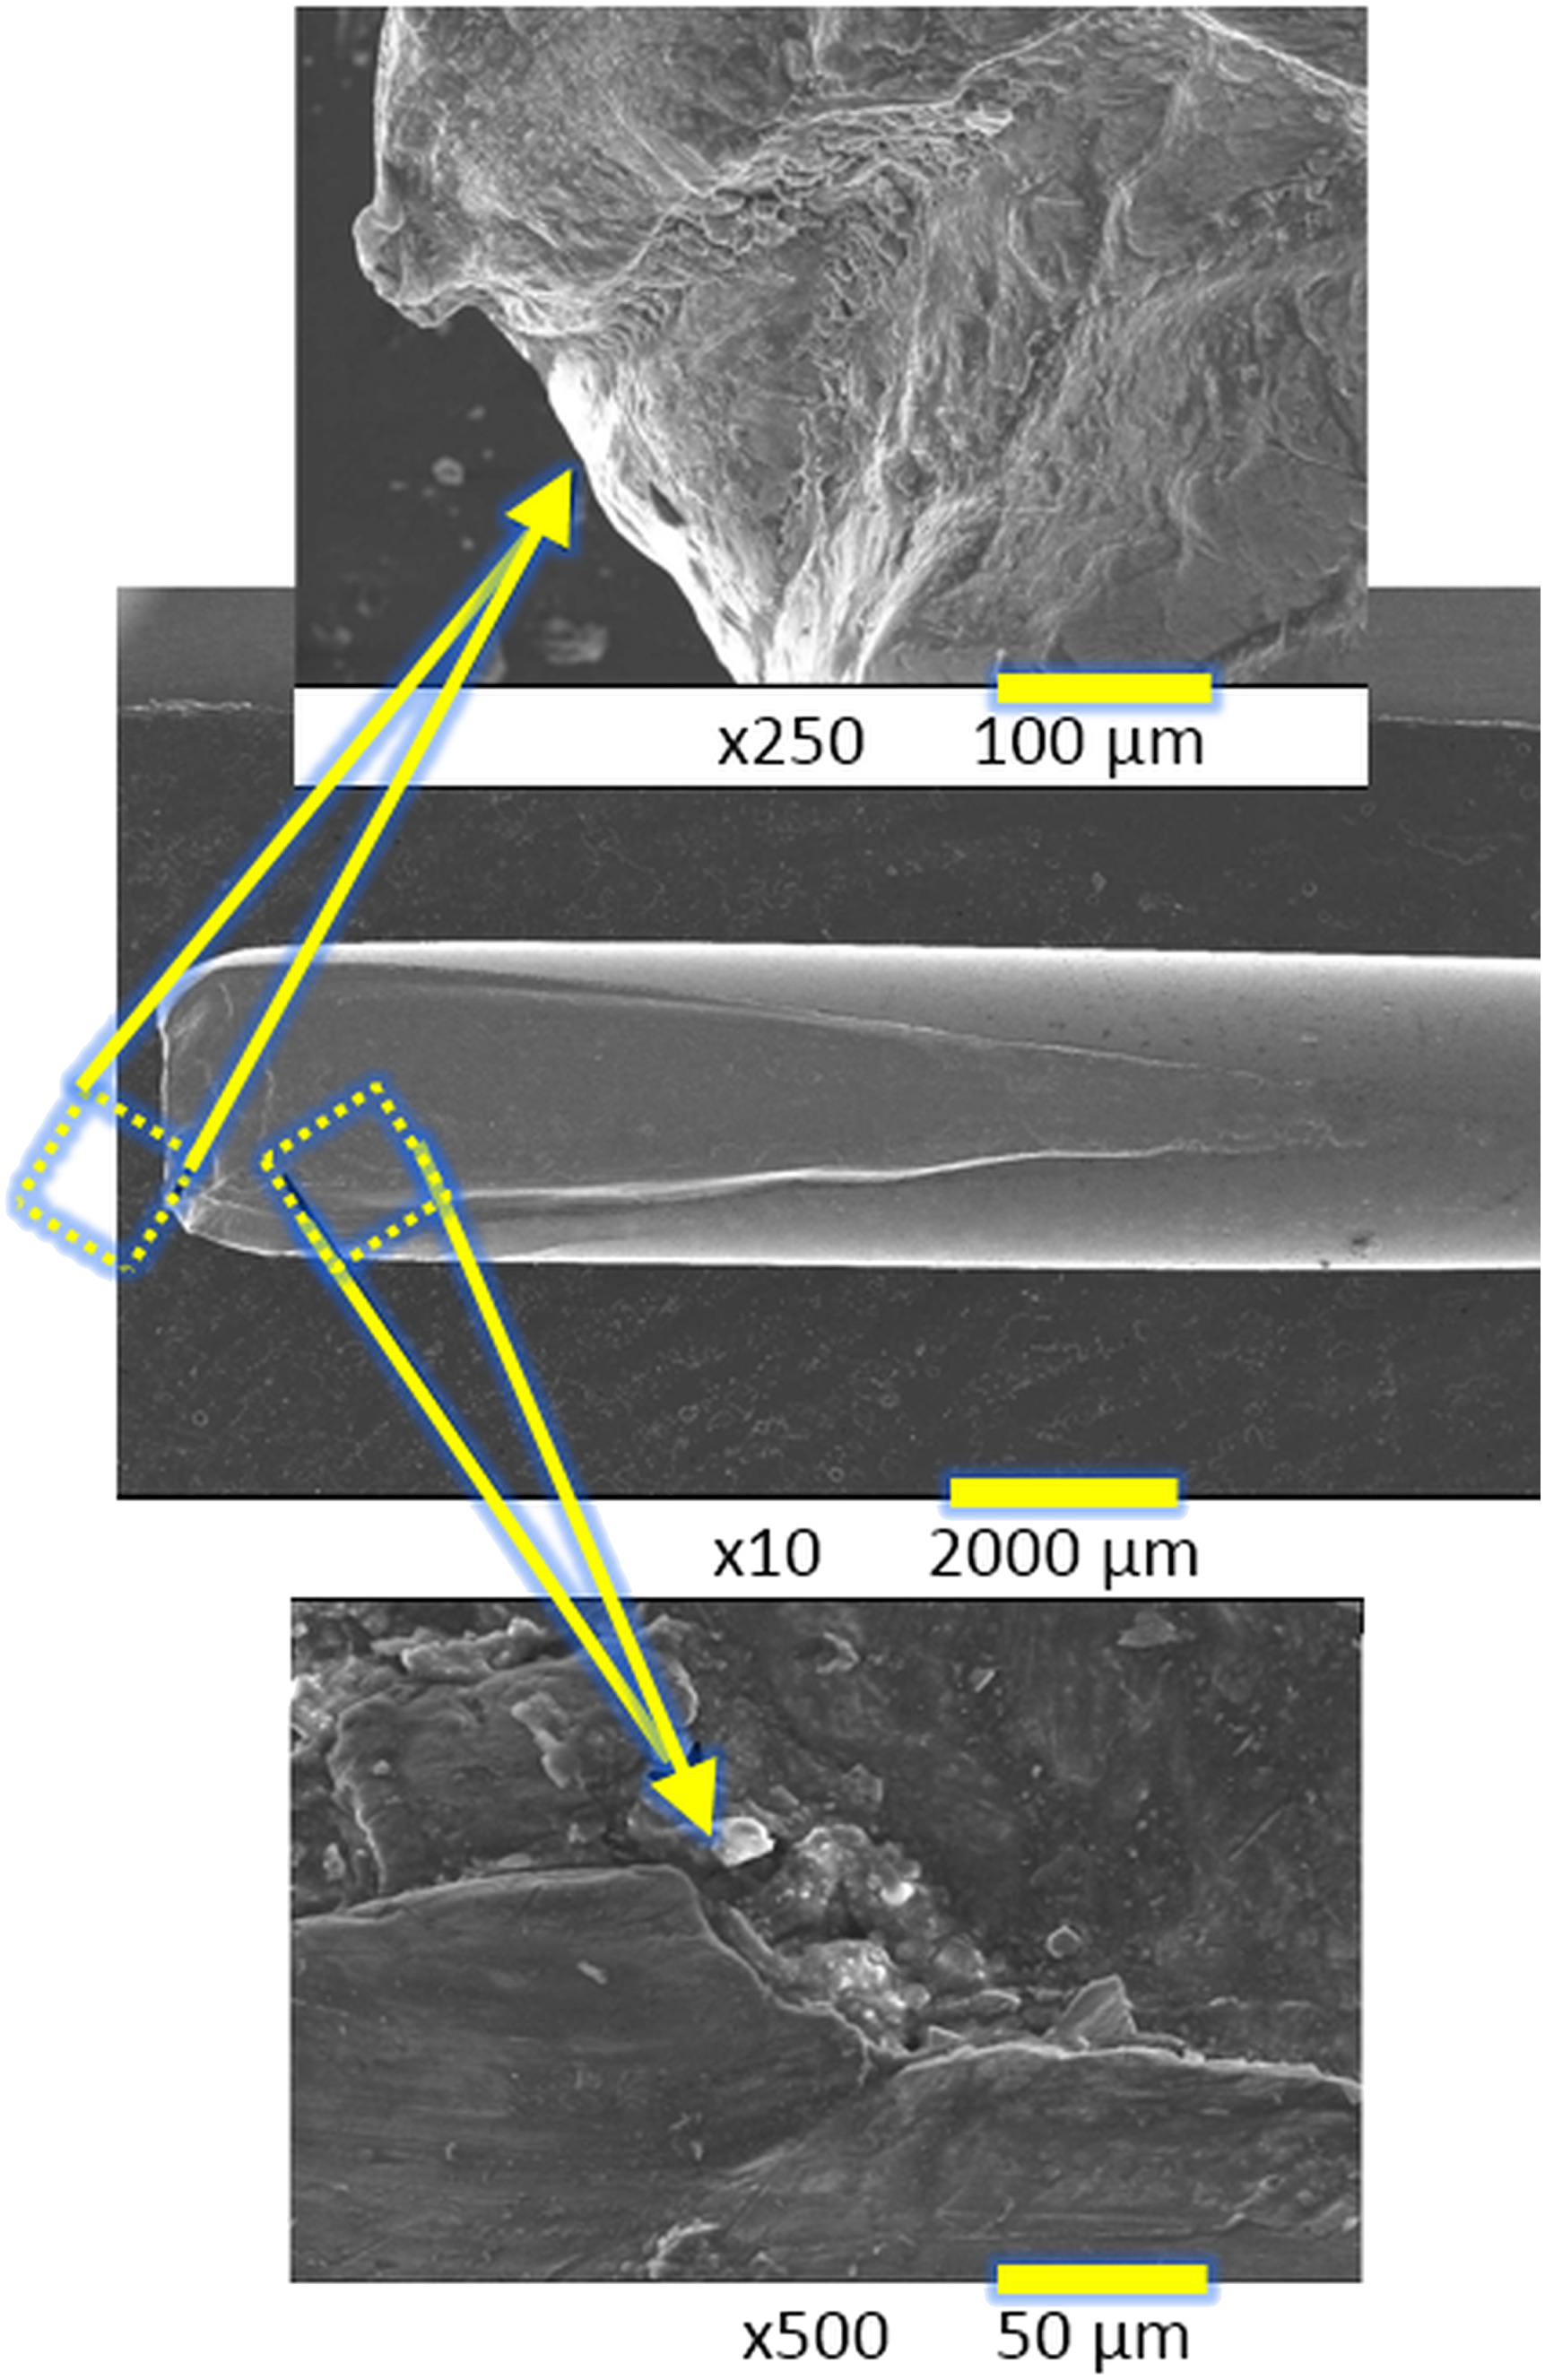
\includegraphics[width=0.7\textwidth]{Figuras/Karabay_2018_fig07_metal_oxide_accumulation.jpg}
    \caption{Zona de acumulação de óxido metálico em fio de alumínio, modo característico de falha por interação metal-máquina.}
    \label{fig:karabay_fig07}
    \fonte{\citeonline{karabay2018failure}.}
\end{figure}

No fio esmaltado, os defeitos de fabricação detectáveis por teste de continuidade são organizados em seis classes principais \cite{demiri2014enamel}. As duas primeiras correspondem a defeitos da matéria-prima: defeitos do vergalhão de cobre, sob a forma de \emph{slivers}\footnote{\emph{Slivers} são lascas alongadas parcialmente destacadas da superfície do vergalhão, formadas durante o lingotamento ou a laminação a quente quando dobras superficiais ou partículas de óxido endurecido são pressionadas contra o metal e em seguida estiradas. Permanecem como descontinuidades superficiais embutidas no fio.} e trincas longitudinais geradas no lingotamento e na laminação, e danos da trefilação, sob a forma de riscos e pontos de \emph{copper fines}\footnote{\emph{Copper fines} são partículas finas de cobre desprendidas da superfície do fio pelo atrito com a fieira durante a trefilação. Quando se acumulam na garganta da fieira, comprometem o filme lubrificante, elevam o coeficiente de atrito e marcam a superfície do fio com pontos defeituosos.} compactados na fieira. As demais classes são específicas da etapa de esmaltação. Contaminação do fio nu por resíduos da solução de trefilação ou por partículas conduzidas até o aplicador pode provocar falhas de continuidade ao se fundir à superfície de cobre. Danos físicos ao filme já curado, como cavidades e arranhões, decorrem do contato do fio com objetos duros ou polias durante o manuseio. Contaminantes aéreos no interior do forno de cura, incluindo flocos queimados de esmalte e partículas de óxido de cobre, ficam embutidos no filme em formação e geram pontos defeituosos. Por fim, defeitos da própria aplicação do verniz produzem bolhas no filme, atribuídas a sujeira ou partículas duras não filtradas pela solução, e \emph{pinholes}\footnote{\emph{Pinholes} são micro-orifícios passantes no filme de esmalte, em geral menores que 100~\textmu m, originados por molhamento inadequado da superfície do fio pela solução resinosa. Expõem o cobre subjacente e produzem falha dielétrica localizada.}, atribuídos a molhamento inadequado do fio na passagem pela solução. A Tabela~\ref{tab:defeitos_fios_esmaltados} sintetiza os principais tipos de defeitos discutidos nesta seção, organizados por característica observável e origem típica, e serve como referência rápida para a discussão metodológica do capítulo seguinte.

\begin{table}[htbp]
    \centering
    \footnotesize
    \caption{Tipos de defeitos associados a fios esmaltados.}
    \label{tab:defeitos_fios_esmaltados}
    \begin{tabularx}{\textwidth}{
        >{\raggedright\arraybackslash}p{0.22\textwidth}
        >{\raggedright\arraybackslash}X
        >{\raggedright\arraybackslash}X
    }
        \toprule
        \textbf{Defeito} & \textbf{Característica principal} & \textbf{Origem típica} \\
        \midrule
        Bolhas no esmalte               & Protuberâncias ou cavidades na camada isolante.                    & Sujeira, ar ou partículas de gel retidas na solução. \\
        Vazios na camada base           & Regiões internas sem preenchimento adequado no revestimento.       & Aplicação irregular ou aprisionamento de solvente. \\
        \emph{Pinholes}                 & Micro-orifícios passantes no filme isolante.                       & Molhamento inadequado do fio pela solução. \\
        Partículas de gel               & Inclusões duras ou pontos elevados no esmalte.                     & Filtragem insuficiente ou degradação polimérica. \\
        Contaminantes aéreos            & Partículas estranhas embutidas no revestimento.                    & Flocos queimados, óxidos ou impurezas no forno de cura. \\
        Riscos e sulcos                 & Marcas lineares ou raspagens no \emph{topcoat}.                    & Contato com guias, manuseio ou embalagem. \\
        \emph{Tracking}                 & Cicatrizes longas ao longo do fio.                                 & Esmalte parcialmente curado em contato com polias. \\
        Cavitação do filme              & Crateras pequenas na superfície do esmalte.                        & Impacto contra objeto rígido durante cura ou manuseio. \\
        Trincas e \emph{slivers} no cobre & Descontinuidades longitudinais no substrato metálico.            & Defeitos de laminação, fundição ou óxidos no cobre. \\
        Dano por trefilação             & Irregularidade contínua no cobre antes da esmaltação.              & Lubrificação inadequada ou matriz gasta. \\
        Fissuras por deformação         & Abertura de falhas no esmalte após dobra ou tração.                & Esforço mecânico sobre defeitos preexistentes. \\
        Rompimento do condutor          & Quebra do fio por concentração de tensão em defeitos do metal.     & Porosidade, inclusões, óxidos ou dano metal-máquina. \\
        \bottomrule
    \end{tabularx}
    \fonte{Adaptado de \citeonline{demiri2014enamel}. A categoria rompimento do condutor usa \citeonline{karabay2018failure} como referência complementar para mecanismos metalúrgicos de quebra.}
\end{table}

% TODO: recortar Fig 30 (pinhole) e Fig 28 (gel/bolhas) da pagina 34 do Demiri (arquivo Demiri_2014_page34_fig28_gel_fig29_voids_fig30_pinhole.png na pasta revisao_literatura). Salvar como Demiri_2014_fig30_pinhole.jpg e Demiri_2014_fig28_gel_bolhas.jpg em vmdi/Figuras e descomentar o bloco abaixo.
% \begin{figure}[htbp]
%     \centering
%     \includegraphics[width=0.7\textwidth]{Figuras/Demiri_2014_fig30_pinhole.jpg}
%     \caption{Pinhole no filme de esmalte do fio de cobre.}
%     \label{fig:demiri_pinhole}
%     \fonte{\citeonline{demiri2014enamel}.}
% \end{figure}

A coexistência desses mecanismos justifica a dificuldade central enfrentada pela operação: um mesmo rompimento pode ter origem na matéria-prima, no equipamento ou em uma combinação dos dois, e as evidências visuais imediatamente disponíveis após o evento não são suficientes para discriminar entre essas hipóteses. A análise sistemática desse fenômeno orienta a investigação para os dados que a operação registra ao longo do processo, apresentados na Seção~\ref{sec:dados_disponiveis}.


\section{Dados disponíveis}
\label{sec:dados_disponiveis}

A análise conduzida nesta pesquisa baseia-se em três conjuntos de dados produzidos pela operação da fábrica. O primeiro consiste em registros operacionais das máquinas das linhas de trefilação e de esmaltação, que reúnem leituras de sensores e parâmetros de processo amostrados continuamente durante a produção. O segundo é o histórico de ordens de produção, que vincula cada janela operacional ao lote de matéria-prima processado, ao fornecedor do vergalhão, ao calibre alvo e às demais variáveis de contexto da ordem. O terceiro corresponde aos eventos de rompimento registrados durante a produção, com informações sobre a máquina, o momento do evento e o material em processo.

Um aspecto central do problema é a ausência de rótulos sobre a causa de cada rompimento. Os eventos são registrados, mas não vêm acompanhados de uma atribuição padronizada da origem provável, isto é, se o rompimento decorreu de defeito de matéria-prima, de falha de equipamento ou de efeito combinado dos dois. Essa ausência de rótulo impede o uso direto de abordagens supervisionadas de aprendizado de máquina sobre o evento em si \cite{chandola2009anomaly} e justifica a estratégia adotada nesta dissertação, baseada em detecção de anomalias operacionais e em análise estatística histórica como evidências independentes a serem combinadas para inferir a origem provável. Antes de detalhar essas duas famílias, no entanto, é necessário situar a abordagem na tradição mais ampla de apoio à decisão técnica em manufatura, revisada na Seção~\ref{sec:diagnostico}.


\section{Diagnóstico de falhas, manutenção e qualidade}
\label{sec:diagnostico}

A tradição de apoio à decisão técnica em manufatura organiza-se em torno de três famílias de ferramentas, complementares em escopo: instrumentos de catalogação preventiva de modos de falha, métodos de análise retrospectiva de causa após um evento e técnicas de monitoramento estatístico contínuo do processo. Esta seção revisa brevemente a contribuição característica de cada família e expõe as limitações que, em conjunto, motivam a busca por abordagens orientadas a dados, discutidas nas Seções~\ref{sec:anomalias} e \ref{sec:estatistica_historica}.

A \emph{Failure Mode and Effects Analysis} (FMEA) é uma metodologia estruturada para enumerar previamente os modos de falha possíveis de um processo ou produto, atribuindo a cada modo uma estimativa de severidade, ocorrência e detectabilidade. Da multiplicação desses três valores resulta o \emph{Risk Priority Number} (RPN), que orienta a priorização de ações corretivas. A técnica surgiu em aplicações aeroespaciais e militares na década de 1960 e foi sistematizada para uso industrial, em particular no setor automotivo, sob padronizações reconhecidas internacionalmente \cite{aiagvda2019fmea,stamatis2003fmea}. Sua principal limitação é o caráter manual e estático: depende do que a equipe de especialistas consegue antecipar a partir do conhecimento prévio do processo, e a tabela resultante envelhece rapidamente quando a operação evolui ou novos modos de falha emergem.

A Análise de Causa Raiz (\emph{Root Cause Analysis}, RCA) reúne técnicas para investigar retrospectivamente a origem provável de um evento indesejado, partindo da manifestação observada e descendo até causas básicas \cite{mobley1999rootcause,doggett2005rootcause}. Métodos comuns incluem os Cinco Porquês, o diagrama de Ishikawa e a análise por árvore de falhas (\emph{Fault Tree Analysis}, FTA), esta última uma extensão formal que combina causas elementares por lógica booleana e é mais frequente em domínios de segurança crítica \cite{vesely1981faulttree,ericson1999faulttree}. Em ambiente produtivo, o \sigla{RCA} é conduzido por engenheiros e operadores após um incidente relevante, e sua qualidade depende da disponibilidade de informações sobre o evento e da experiência da equipe envolvida. Tal como o \sigla{FMEA}, o \sigla{RCA} não absorve dados sensoriais de forma sistemática: produz diagnóstico por consenso humano, caso a caso, em vez de vigiar o processo continuamente.

O Controle Estatístico de Processo (\emph{Statistical Process Control}, SPC, ou CEP), por sua vez, oferece monitoramento contínuo de variáveis de processo ao longo do tempo. O instrumento central é a carta de controle, na qual os valores observados de uma variável são comparados a limites estatísticos derivados da variabilidade natural do processo. Cartas de Shewhart, cartas de soma acumulada (CUSUM) e cartas de média móvel exponencialmente ponderada (EWMA) representam as principais famílias, com sensibilidades distintas a desvios abruptos e a deslocamentos sustentados \cite{montgomery2019statistical}. Índices de capabilidade como $C_p$ e $C_{pk}$ vinculam a variação natural do processo à tolerância de projeto. Extensões multivariadas, como a estatística $T^2$ de Hotelling e suas versões temporais MEWMA e MCUSUM, foram propostas para situações em que múltiplas variáveis são monitoradas simultaneamente \cite{hotelling1947multivariate,lowry1992multivariate}. Na prática, contudo, o \sigla{CEP} é aplicado majoritariamente de forma univariada, com pressupostos de normalidade e independência temporal que se tornam frágeis quando o processo é caracterizado por dezenas de sensores correlacionados, amostrados em alta frequência e sob regimes operacionais não estacionários.

Tomadas em conjunto, \sigla{FMEA}, \sigla{RCA} e \sigla{CEP} constituem a linguagem comum com que a indústria estrutura diagnóstico e qualidade há décadas. Suas limitações para o cenário desta dissertação são complementares. As duas primeiras ferramentas dependem de rotulagem manual de causa, conduzida por especialistas e difícil de escalar para o volume de eventos registrados continuamente. A terceira escala em frequência, mas estagna em dimensionalidade e em flexibilidade estatística. Na fábrica analisada, a aplicação do \sigla{FMEA} e do \sigla{RCA} depende da intervenção pontual de operadores experientes após cada incidente relevante, prática que não acompanha o ritmo de geração de dados pelas máquinas e motiva a busca por abordagens automatizadas, capazes de combinar evidências independentes, examinadas nas Seções~\ref{sec:anomalias} e \ref{sec:estatistica_historica}.


\section{Detecção de anomalias em dados industriais}
\label{sec:anomalias}

A detecção de anomalias compreende o conjunto de técnicas dedicadas a identificar observações que se afastam do padrão esperado em um conjunto de dados. A literatura distingue três tipos canônicos. Anomalias pontuais correspondem a observações isoladas que diferem do restante do conjunto. Anomalias contextuais são observações que só se mostram anômalas quando avaliadas em relação ao seu contexto, como uma leitura de temperatura normal no inverno mas atípica no verão. Anomalias coletivas, por sua vez, são grupos de observações que formam um padrão atípico mesmo que cada elemento isolado pareça normal \cite{chandola2009anomaly}. A escolha do método depende também do regime de aprendizado disponível: técnicas supervisionadas exigem rótulos de normalidade e anomalia para cada amostra de treino, técnicas semi-supervisionadas exigem apenas exemplos da classe normal, e técnicas não supervisionadas operam sem rótulo algum, identificando padrões raros ou pouco frequentes a partir da estrutura intrínseca dos dados. No cenário desta dissertação, em que rompimentos são registrados sem atribuição de causa, o regime não supervisionado é o único viável e orienta toda a discussão da seção.

Quando o objeto de detecção é uma linha de produção, a tarefa adquire complicadores específicos. Os sensores registram dezenas de variáveis simultaneamente, com correlações estruturais entre si que refletem o acoplamento físico do processo, como a relação direta entre a temperatura do forno e a velocidade da linha. O regime de operação não é estacionário: os valores de referência operacional mudam ao longo do dia, materiais distintos são processados em sequência e a linha passa por transientes legítimos como rampas de partida e trocas de produto, que precisam ser distinguidos de anomalias reais. Além disso, o conceito de comportamento normal evolui ao longo do tempo, fenômeno conhecido como deriva conceitual (\emph{concept drift}), o que exige que o modelo seja capaz de se adaptar sem comprometer a sensibilidade \textcolor{red}{[ref: revisão sobre concept drift, p. ex. Gama et al. 2014 ou Lu et al. 2018]}. Esses fatores tornam abordagens univariadas e estacionárias, como as cartas de controle clássicas discutidas na Seção~\ref{sec:diagnostico}, insuficientes para o tipo de dado disponível.

As técnicas de detecção de anomalias se organizam em famílias distintas conforme o princípio de discriminação que adotam. Métodos estatísticos clássicos, como a estatística $T^2$ de Hotelling apresentada na Seção~\ref{sec:diagnostico}, modelam a distribuição esperada dos dados e sinalizam como anômalas as observações cuja verossimilhança fica abaixo de um limiar pré-estabelecido. Métodos baseados em densidade, como o \emph{Local Outlier Factor} (LOF), comparam a densidade local de cada ponto com a densidade de seus vizinhos no espaço de atributos, sinalizando como anômalas as observações que residem em regiões esparsas \textcolor{red}{[ref: Breunig et al. 2000 (\emph{LOF: Identifying Density-Based Local Outliers}) e Aggarwal 2017 (\emph{Outlier Analysis})]}. Métodos baseados em isolamento exploram a observação de que pontos anômalos tendem a ser isolados em poucos cortes aleatórios do espaço, dispensando estimativas explícitas de densidade ou distribuição. Modelos profundos, como autoencoders e redes recorrentes do tipo \emph{Long Short-Term Memory} (LSTM), oferecem alternativas para situações em que padrões complexos e relações temporais de longo prazo precisam ser capturados, ao custo de maior demanda computacional e de dados de treino \textcolor{red}{[ref: Pang et al. 2021 (\emph{Deep Learning for Anomaly Detection: A Review}), ACM Computing Surveys]}. A escolha entre famílias depende de fatores como dimensionalidade, volume de dados, requisitos de interpretabilidade e custo computacional.

Dentre as famílias apresentadas, o método de isolamento conhecido como \emph{Isolation Forest} é o adotado nesta dissertação \textcolor{red}{[ref: Liu, Ting e Zhou 2008 (\emph{Isolation Forest}), ICDM, ou Liu et al. 2012 (\emph{Isolation-Based Anomaly Detection}), TKDD]}. O algoritmo opera construindo um \emph{ensemble} de árvores binárias em que cada divisão é feita selecionando aleatoriamente um atributo e um valor de corte dentro do intervalo observado desse atributo. Sob essa partição aleatória, pontos anômalos tendem a ser separados do conjunto principal em poucos níveis da árvore, enquanto pontos normais exigem partições sucessivas até serem isolados. O escore de anomalia atribuído a cada observação deriva da profundidade média de isolamento ao longo das árvores do ensemble, normalizado para o intervalo entre zero e um, com valores próximos de um indicando alta probabilidade de anomalia. O método se caracteriza pela escalabilidade em alta dimensionalidade, pela ausência de pressupostos paramétricos sobre a distribuição dos dados e pelo custo computacional linear no tamanho do conjunto. Os principais hiperparâmetros são o número de árvores do ensemble, o tamanho da sub-amostra usada para construir cada árvore e o parâmetro de contaminação esperada, que define o limiar de classificação entre escores normais e anômalos.

A avaliação de detectores de anomalia treinados sem rótulo apresenta dificuldade própria. Métricas clássicas como precisão, \emph{recall} e área sob a curva ROC (\emph{Receiver Operating Characteristic}) dependem da existência de uma verdade de referência (\emph{ground truth}) que indique quais observações são efetivamente anômalas, condição não satisfeita no cenário aqui considerado. A literatura propõe estratégias alternativas para lidar com essa limitação. Uma é a avaliação por especialistas, que examinam manualmente um subconjunto das observações sinalizadas pelo modelo e julgam se o sinal é coerente com o comportamento esperado da operação. Outra é a comparação com eventos conhecidos, na qual os escores produzidos pelo modelo são confrontados com registros de incidentes documentados a posteriori. A análise de consistência interna verifica se observações próximas no tempo ou no espaço de atributos recebem escores compatíveis, sob a hipótese de que a transição entre estados operacionais é gradual. Estudos de robustez, por fim, treinam e testam o modelo com diferentes recortes e parametrizações para avaliar a estabilidade dos resultados frente a variações de calibragem \textcolor{red}{[ref: Goldstein e Uchida 2016 (\emph{A Comparative Evaluation of Unsupervised Anomaly Detection Algorithms}) e Pang et al. 2021]}. Essas estratégias não substituem rótulos, mas oferecem evidências indiretas sobre o comportamento do modelo.

A literatura registra aplicações de detecção de anomalia em diversos domínios de manufatura, incluindo monitoramento preditivo de máquinas, controle de qualidade de produto e identificação de desvios de processo \textcolor{red}{[ref: surveys de manutenção preditiva e Indústria 4.0, p. ex. Carvalho et al. 2019 ou Zhao et al. 2019]}. No contexto da fabricação de fios esmaltados, contudo, técnicas isoladas de anomalia apresentam limite estrutural: o modelo é capaz de sinalizar que o comportamento operacional da máquina se afastou do esperado em determinado intervalo, mas é incapaz, por construção, de atribuir esse desvio a uma causa específica. Quando o rompimento decorre de defeito de matéria-prima formado antes do início da linha analisada, conforme discutido na Seção~\ref{sec:problema_rompimentos}, os sensores podem nem registrar comportamento atípico, pois a falha viaja embutida no fio e se manifesta apenas em um ponto físico distante de sua origem. Além disso, a detecção de anomalias por séries operacionais ignora um eixo de informação relevante: o histórico estatístico de rompimentos por lote, material, fornecedor e máquina, capaz de revelar padrões sistemáticos que escapam à análise no nível do evento individual. Essa lacuna motiva a discussão da Seção~\ref{sec:estatistica_historica}.


\section{Análise estatística histórica de falhas}
\label{sec:estatistica_historica}

% Função retórica: apresentar a família de técnicas que
% sustenta o Pilar MP.
% RQ3.
% Conteúdo a desenvolver:
%   - Taxa de falha, exposição operacional e risco relativo.
%   - Recorrência por lote, material, fornecedor e máquina.
%   - Efeito de lote e variabilidade entre fornecedores.
%   - Indicadores de qualidade de matéria-prima em
%     processo contínuo.
% Conclui apontando que estatística histórica isolada não
% captura desvio operacional em janela curta e depende de
% agregação que pode atrasar o diagnóstico.


\section{Sistemas híbridos e explicabilidade}
\label{sec:hibridos_xai}

% Função retórica: mostrar que combinar as duas famílias é a
% direção promissora, mas pouco consolidada no domínio de fios
% esmaltados, e apontar a lacuna.
% RQ2 e RQ4.
% Conteúdo a desenvolver:
%   - Estratégias de combinação (regras, ensemble, fusão de
%     evidências, sistemas em camadas).
%   - Importância de resultados interpretáveis em chão de
%     fábrica.
%   - Interpretabilidade aplicada a manutenção, qualidade e
%     engenharia.
% Conclui com o parágrafo da lacuna:
%   - Existe maturidade nas duas famílias isoladas.
%   - Há trabalhos pontuais de integração em outros domínios.
%   - Falta uma arquitetura híbrida e explicável aplicada ao
%     domínio específico de fios esmaltados, com regra de
%     cruzamento entre máquinas para diferenciar falha de
%     equipamento de suspeita de matéria-prima.
%   - Essa lacuna motiva o capítulo seguinte.
